\section{Spectral Clustering}

\begin{frame} 
  \frametitle{References}

    \begin{thebibliography}{99}
      \setbeamertemplate{bibliography item}[book]

    \bibitem{DS}{DS} David Sontag's Lecture
    \newblock \url{http://people.csail.mit.edu/dsontag/courses/ml13/slides/lecture16.pdf}
    
    \bibitem[VLB]{VLB} A Tutorial on Spectral Clustering, 
    \newblock \textcolor{black}{Ulrike von Luxburg}

    \end{thebibliography}

\end{frame}

\begin{frame}
  \frametitle{Spectral Clustering}
  
  \begin{block}{Principle: graph-based transformation prior to clustering} 
    \begin{enumerate}
      \item Build a similarity with a weighted graph of the data 
      \item Use the spectral property of this similarity (graphical Laplacian \rsa kernel)
      \item Apply clustering (e.g., k-means) to the transformed data 
      \item 
    \end{enumerate}
  \end{block}

  \begin{figure}[ht]
    \centering
    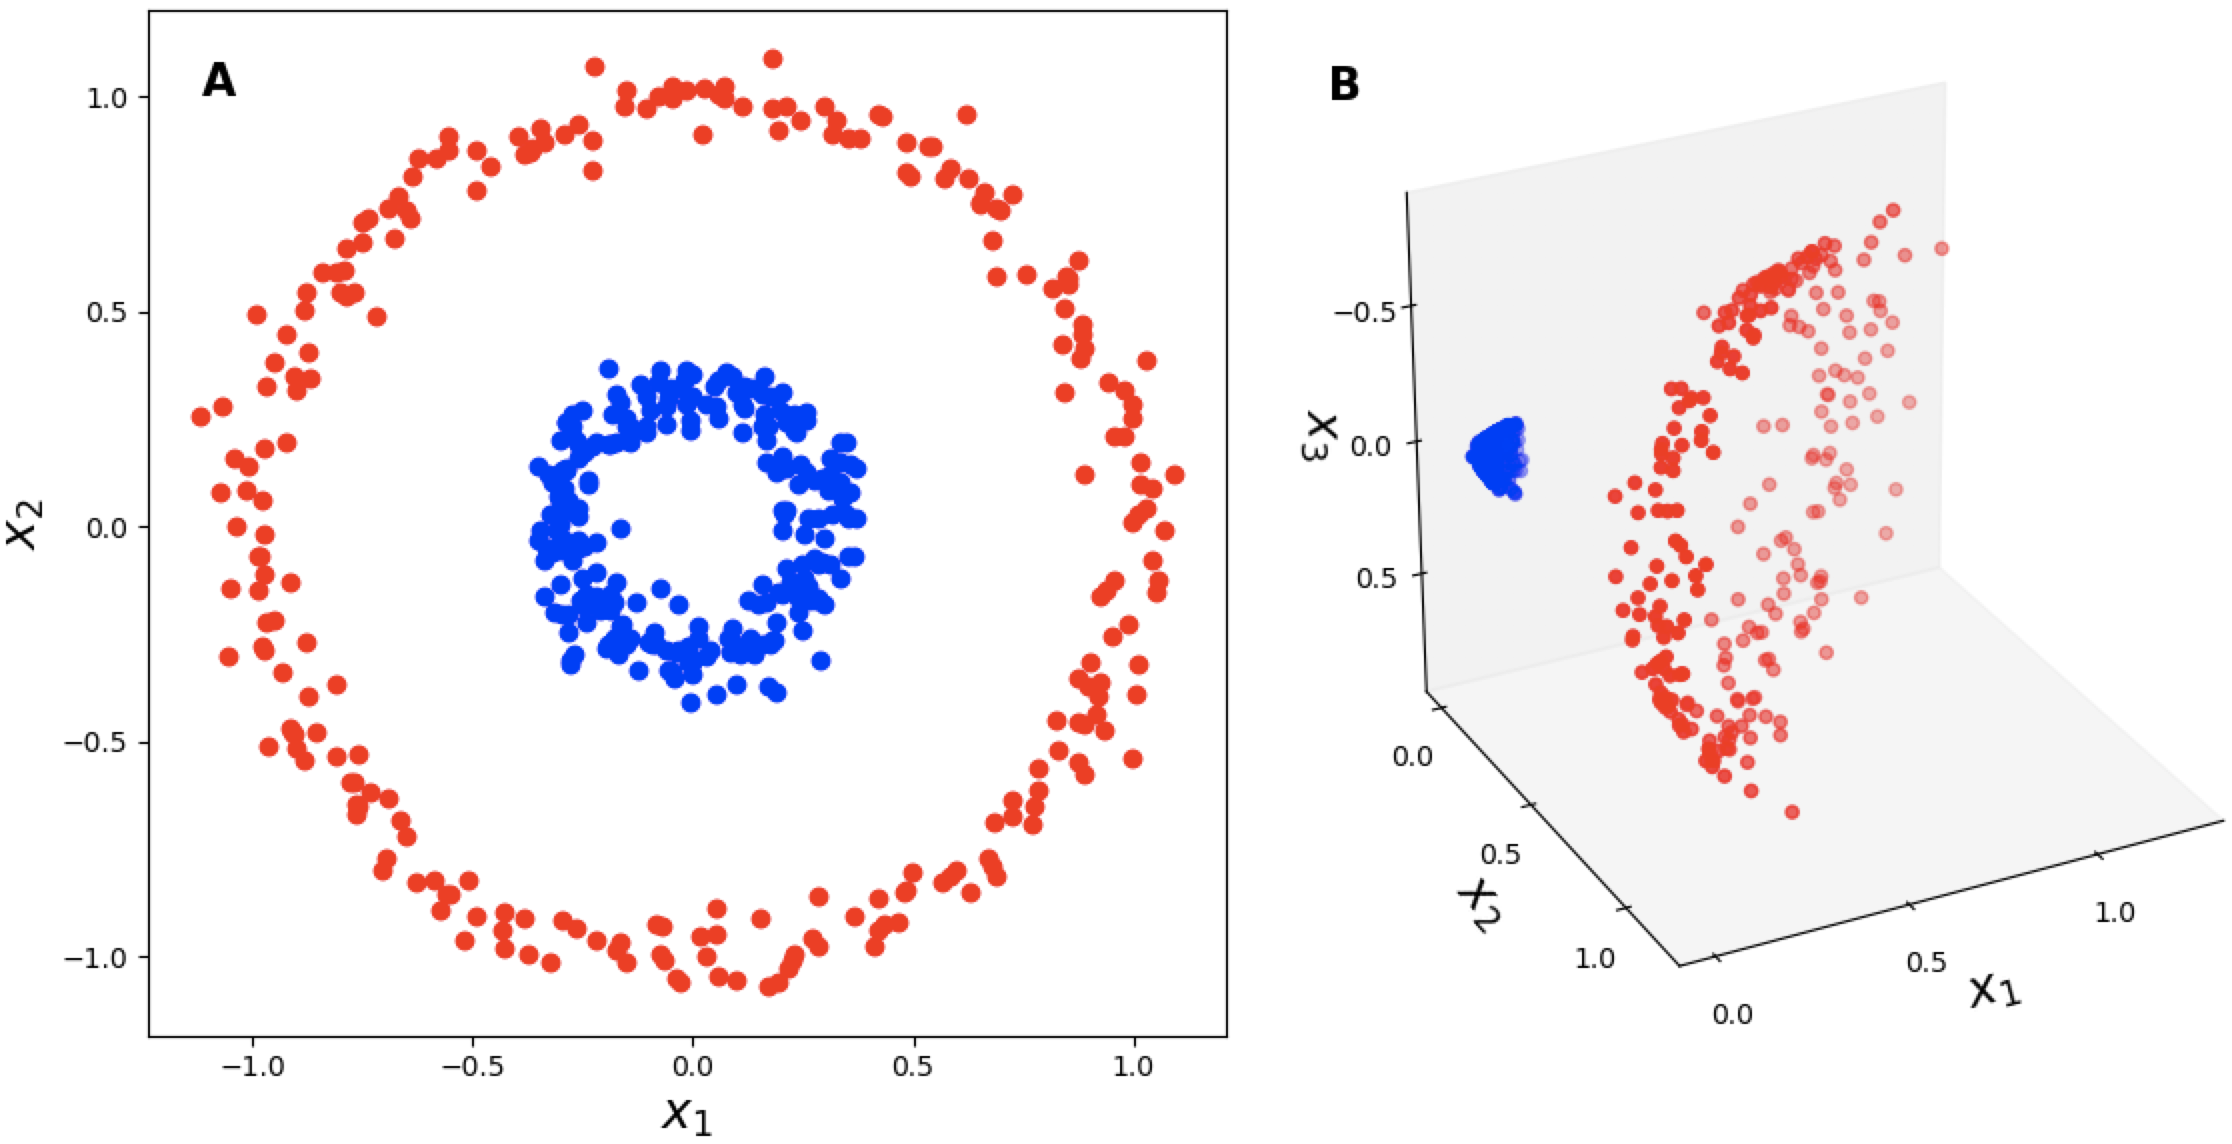
\includegraphics[height=4cm]{figures/kernel_trick2}
    \caption{Performing clustering after non-linear transformation of the data }
  \end{figure}

\end{frame}

\begin{frame}
  \frametitle{Adjacency matrix and list of edges}

  \begin{definition}[Adjacency matrix \only<1>{(binary graph)}\only<1>{(weighted graph)} ]
    The connectivity of  $\clG = (\clV,\clE)$ is captured by the $|\clV|\times |\clV|$ matrix $\bA$:
    \[
      (\bA)_{ij} = \begin{cases}
      \only<1>{(binary graph)}\only<1>{(w_{ij})}  & \text{ if } i \sim j,\\
      0  & \text{otherwise}.
      \end{cases}
    \]
  \end{definition}

  \begin{proposition}
    The degrees of $\clG$ are then simply obtained as the row-wise and/or column-wise sums of $\bA$.
  \end{proposition}

\end{frame}

\begin{frame}
  \frametitle{Incidence matrix}

  \begin{definition}[Incidence matrix]
    The connectivity of $\clG = (\clV,\clE)$ is captured by the $|\clV|\times |\clE|$ matrix $\bB$:
    \[
      (\bB)_{ij} = \begin{cases}
      1  & \text{ if $i$ is incident to edge $j$},\\
      0  & \text{otherwise}.
      \end{cases}
    \]
  \end{definition}

  \begin{proposition}[Relationship]
    Let $\tilde\bB$ be a modified \alert{signed} version of $\bB$ where $\tilde{\! B}_{ij}= 1/-1$ if $i$ is incident to $j$ as tail/head. Then
    \[
      \tilde \bB \tilde \bB^\intercal = \bD - \bA,
    \]
    where $\bD = \diag(\set{d_i, i\in\clV})$ is the diagonal matrix of degrees. 
  \end{proposition}

\end{frame}

\begin{frame}
  \frametitle{Graph Laplacian}

  \begin{definition}[(Un-normalized) Laplacian]
    The Laplacian matrix $\bL$, resulting from the modified incidence matrix $\tilde\bB$ $\tilde{\! B}_{ij}= 1/-1$ if $i$ is incident to $j$ as tail/head, is defined by 
    \[
      \bL = \tilde \bB \tilde \bB^\intercal = \bD - \bA,
    \]
    where $\bD = \diag(d_i, i\in\clV)$ is the diagonal matrix of degrees. 
  \end{definition}

  \begin{block}{Remark}
    \begin{itemize}
    \item $\bL$ is called the graph Laplacian (by analogy to continuous Laplacian).
    \item Spectrum of $\bL$ has much to say about the structure of the graph $\clG$.
    \end{itemize}
  \end{block}

\end{frame}

\begin{frame}
  \frametitle{Graph Laplacian: spectrum}

  \begin{proposition}[Spectrum of $\bL$]
    The $n\times n$ matrix $\bL$ has the following properties:
    \[
      \bx^\top \bL \bx = \frac{1}{2} \sum_{i,j} A_{ij} (x_i - x_j)^2, \quad \forall \bx\in\Rset^n .
    \]
    \vspace{-.25cm}
    \begin{itemize}
      \item $\bL$ is a symmetric, positive semi-definite matrix,
      \item  the smallest eigenvalue is $0$ with associated eigenvector $\mathbf{1}$.
      \item $\bL$ has $n$ positive eigenvalues $0=\lambda_1<\dots <\lambda_n$. 
    \end{itemize}  
  \end{proposition}

  \begin{corollary}[Spectrum and Graph]
    \vspace{-.25cm}
    \begin{itemize}
      \item The multiplicity of the first eigen value ($0$) of $\bL$ determines the number of connected components in the graph.
      \item The larger the second non trivial eigenvalue, the higher the connectivity of $\clG$.
    \end{itemize}  
  \end{corollary}

\end{frame}

\begin{frame}
  \frametitle{Some variants}

  \begin{definition}[(Normalized) Laplacian]
    The normalized Laplacian matrix $\bL$ is defined by 
    \[
      \bL_N = \bD^{-1/2}\bL\bD^{-1/2} = \bI - \bD^{-1/2} \bA \bD^{-1/2}.
    \]
  \end{definition}
  
  \vfill

  \begin{definition}[(Absolute) Graph Laplacian]
    The absolute Laplacian matrix $\bL_{abs}$ is defined by 
    \[
      \bL_{abs} = \bD^{-1/2}\bA\bD^{-1/2} = \bI - \bL_N,
    \]
    with eigenvalues $1-\lambda_n \leq \dots \leq 1-\lambda_2 \leq 1-\lambda_1 = 1$, where $0=\lambda_1\leq \dots \leq \lambda_n$ are the eigenvalues of $\bL_N$.
  \end{definition}

\end{frame}

\begin{frame}
  \frametitle{Spectral Clustering}
    
  \begin{block}{Principle}
  
  \begin{enumerate}
    \item Use the spectral property of $\bL$ to perform clustering in the eigen space \medskip
    \item If the network have $K$ connected components, the first $K$ eigenvectors are $\mathbf{1}$ span the eigenspace associated with eigenvalue $0$ \medskip
    \item Applying a simple clustering algorithm to the rows of the $K$ first eigenvectors separate the components
  \end{enumerate}
  $\rightsquigarrow$ This principle generalizes to a graph with a single component: spectral clustering tends to separates groups of nodes which are highly connected together
  
  \end{block}
  
\end{frame}

\begin{frame}
  \frametitle{Normalized Spectral Clustering}
  \framesubtitle{by Ng, Jordan and Weiss (2002)}

\begin{algorithm}[H]
  \KwIn{Adjacency matrix and number of classes $Q$}
  \BlankLine\BlankLine
  \DontPrintSemicolon
  
  Compute the normalized graph Laplacian $\mathbf{L}$\;
  Compute the eigen vectors of $\mathbf{L}$ associated with the $Q$ \alert{smallest eigenvalues}\;
  Define $\mathbf{U}$,  the $n\times Q$ matrix  that encompasses these $Q$ vectors \;
  Define $\tilde{\mathbf{U}}$, the row-wise normalized version of $\mathbf{U}$: $ \tilde{u}_{ij} = \frac{u_{ij}}{\| \mathbf{U}_i\|_2}$\;
  Apply k-means to $(\tilde{\mathbf{U}}_i)_{i=1,\dots,n}$

  \BlankLine\BlankLine
  \KwOut{vector of classes $\mathbf{C}\in \mathcal{Q}^n$, such as  $C_i = q$ if $i\in q$}

\end{algorithm}

  \vfill

  \begin{block}{Remarks}
    \begin{itemize}
      \item implemented during today's lab
      \item also apply to no graphical data!
    \end{itemize}
  \end{block}
  
\end{frame}
% 
% \begin{frame}
%   \frametitle{Absolute Spectral Clustering}
% 
% \begin{algorithm}[H]
%   \KwIn{Adjacency matrix and number of classes $Q$}
%   \BlankLine\BlankLine
%   \DontPrintSemicolon
% 
%   Compute the graph Laplacian $\mathbf{L}_{abs}$\;
%   Compute the eigen vectors of $\mathbf{L}_{abs}$ associated with the $Q$ \alert{largest} absolute eigenvalues\;
%   Define $\mathbf{U}$,  the $p\times Q$ matrix  that encompasses these $Q$ vectors \;
%   Apply k-means to $(\mathbf{U}_i)_{i=1,\dots,p}$
% 
%   \BlankLine\BlankLine
%   \KwOut{vector of classes $\mathbf{C}\in \mathcal{Q}^p$, such as  $C_i = q$ if $i\in q$}
% 
%   \caption{Spectral Clustering by Rohe et al. (2011)}
% \end{algorithm}
% 
% \end{frame}


\begin{frame}[fragile,allowframebreaks]
  \frametitle{Crabs: Fielder vector and eigenvalue}

\begin{knitrout}
\definecolor{shadecolor}{rgb}{0.969, 0.969, 0.969}\color{fgcolor}\begin{kframe}
\begin{alltt}
\hlstd{graph_crabs} \hlkwb{<-} \hlstd{crabs} \hlopt \hlkwd{select}\hlstd{(}\hlopt{-}\hlstd{species,} \hlopt{-}\hlstd{sex)} \hlopt
  \hlkwd{t}\hlstd{()} \hlopt \hlkwd{cor}\hlstd{()} \hlopt \hlkwd{graph_from_adjacency_matrix}\hlstd{(}\hlkwc{weighted} \hlstd{=} \hlnum{TRUE}\hlstd{)}
\end{alltt}


{\ttfamily\noindent\bfseries\color{errorcolor}{\#\# Error in crabs \%>\% select(-species, -sex) \%>\% t() \%>\% cor() \%>\% graph\_from\_adjacency\_matrix(weighted = TRUE): could not find function "{}\%>\%"{}}}\begin{alltt}
\hlstd{eigen_crabs} \hlkwb{<-} \hlkwd{graph.laplacian}\hlstd{(graph_crabs)} \hlopt \hlkwd{eigen}\hlstd{()}
\end{alltt}


{\ttfamily\noindent\bfseries\color{errorcolor}{\#\# Error in graph.laplacian(graph\_crabs) \%>\% eigen(): could not find function "{}\%>\%"{}}}\begin{alltt}
\hlstd{fielder_vector} \hlkwb{<-} \hlstd{eigen_crabs}\hlopt{$}\hlstd{vectors[,} \hlkwd{nrow}\hlstd{(crabs)} \hlopt{-} \hlnum{1}\hlstd{]}
\end{alltt}


{\ttfamily\noindent\bfseries\color{errorcolor}{\#\# Error in eval(expr, envir, enclos): object 'eigen\_crabs' not found}}\begin{alltt}
\hlstd{faction} \hlkwb{<-} \hlkwd{factor}\hlstd{(}\hlkwd{paste}\hlstd{(crabs}\hlopt{$}\hlstd{species, crabs}\hlopt{$}\hlstd{sex,} \hlkwc{sep}\hlstd{=}\hlstr{"-"}\hlstd{))}
\end{alltt}


{\ttfamily\noindent\bfseries\color{errorcolor}{\#\# Error in paste(crabs\$species, crabs\$sex, sep = "{}-"{}): object 'crabs' not found}}\begin{alltt}
\hlkwd{par}\hlstd{(}\hlkwc{mfrow} \hlstd{=} \hlkwd{c}\hlstd{(}\hlnum{1}\hlstd{,}\hlnum{2}\hlstd{))}
\hlkwd{plot}\hlstd{(eigen_crabs}\hlopt{$}\hlstd{values[}\hlopt{-}\hlkwd{nrow}\hlstd{(crabs)],} \hlkwc{col} \hlstd{=} \hlstr{"blue"}\hlstd{,} \hlkwc{ylab} \hlstd{=} \hlstr{"Eigenvalues of Graph Laplacian"}\hlstd{)}
\end{alltt}


{\ttfamily\noindent\bfseries\color{errorcolor}{\#\# Error in plot(eigen\_crabs\$values[-nrow(crabs)], col = "{}blue"{}, ylab = "{}Eigenvalues of Graph Laplacian"{}): object 'eigen\_crabs' not found}}\begin{alltt}
\hlkwd{plot}\hlstd{(fielder_vector,} \hlkwc{pch} \hlstd{=} \hlnum{16}\hlstd{,} \hlkwc{xlab} \hlstd{=} \hlstr{"labels"}\hlstd{,}
   \hlkwc{ylab} \hlstd{=} \hlstr{"Fielder vector entry"}\hlstd{,} \hlkwc{col} \hlstd{= faction)}
\end{alltt}


{\ttfamily\noindent\bfseries\color{errorcolor}{\#\# Error in plot(fielder\_vector, pch = 16, xlab = "{}labels"{}, ylab = "{}Fielder vector entry"{}, : object 'fielder\_vector' not found}}\begin{alltt}
\hlkwd{abline}\hlstd{(}\hlnum{0}\hlstd{,} \hlnum{0}\hlstd{,} \hlkwc{lwd} \hlstd{=} \hlnum{2}\hlstd{,} \hlkwc{col} \hlstd{=} \hlstr{"lightgray"}\hlstd{)}
\end{alltt}


{\ttfamily\noindent\bfseries\color{errorcolor}{\#\# Error in int\_abline(a = a, b = b, h = h, v = v, untf = untf, ...): plot.new has not been called yet}}\end{kframe}
\end{knitrout}

\end{frame}
